% !TEX program = pdflatex
\documentclass[11pt]{article}
\usepackage[margin=1in]{geometry}
\usepackage{float,needspace}
\usepackage{amsthm}
\newtheorem{lemma}{Lemma}[section]
\usepackage{microtype,amsmath,amssymb,booktabs,tabularx,array,graphicx,xurl,longtable,placeins,multirow}

\usepackage[table]{xcolor}
\definecolor{MediterraneanBlue}{HTML}{2F88B8}
\definecolor{MediterraneanTeal}{HTML}{4FA58A}
\definecolor{MediterraneanTerra}{HTML}{E57D3F}
\definecolor{MediterraneanSlate}{HTML}{56627A}
\arrayrulecolor{black}
\renewcommand{\arraystretch}{1.12}
\setlength{\aboverulesep}{3pt}
\setlength{\belowrulesep}{3pt}
\setlength{\textfloatsep}{7pt plus 2pt minus 2pt}
\setlength{\intextsep}{8pt plus 2pt minus 2pt}
\renewcommand{\topfraction}{.85}
\renewcommand{\textfraction}{.10}
\renewcommand{\floatpagefraction}{.85}
\widowpenalty=10000
\clubpenalty=10000

\usepackage[font=small,labelfont=bf,skip=4pt]{caption}
\makeatletter
\renewcommand\section{\@startsection{section}{1}{\z@}{-2.2ex \@plus -0.8ex \@minus -.2ex}{1.2ex \@plus .2ex}{\normalfont\Large\bfseries}}
\renewcommand\subsection{\@startsection{subsection}{2}{\z@}{-1.8ex \@plus -0.8ex \@minus -.2ex}{0.9ex \@plus .2ex}{\normalfont\large\bfseries}}
\renewcommand\paragraph{\@startsection{paragraph}{4}{\z@}{1.6ex \@plus .5ex \@minus .2ex}{-1em}{\normalfont\normalsize\bfseries}}
\makeatother
\usepackage[round,authoryear]{natbib}
\usepackage[colorlinks=true,linkcolor=blue,citecolor=blue,urlcolor=blue]{hyperref}
\DeclareUrlCommand\path{\urlstyle{same}}
\setlength{\emergencystretch}{3em}
\newcolumntype{Y}{>{\raggedright\arraybackslash}X}
\newcommand{\JOIN}{\mathsf{JOIN}}\newcommand{\SAFE}{\mathsf{SAFE}}\newcommand{\E}{\mathbb E}
\title{Framing and Inattention in Delegated Choice:\\ Evidence from LLM Agents}
\author{Yuxuan Cai \\ {\normalsize 2200011728} \and Xingyu Peng \\ {\normalsize 2400011746} \and Liang Shan \\ {\normalsize 2300012444}  \and Aolin Zhang \\ {\normalsize 2400010701}}
\date{\small Behavioral Economics (Fall 2026), Track C: AI Behavioral Experiment and Report}
\begin{document}\maketitle
\begin{abstract}
\noindent We test two basic requirements of rational choice in large language model (LLM) agents that choose on people's behalf: invariance to payoff-irrelevant information and full response to opportunity cost. An agent decides whether to join a project that pays off only if a programmed partner also joins, or to take a safe payoff. Starting from the standard decision problem, we model the choice in two steps, valuation and comparison, each with one behavioral parameter: $\kappa$, the extent to which probabilities that should be conditioned away distort the perceived value of joining, and $\theta$, the attention weight on the outside option. Both requirements fail, and both failures lie in the decision procedure rather than in preferences or beliefs. For GPT-6 Luna without reasoning, an uninformative message raises the joining rate by up to 12 percentage points (pp) and an outdated prior by 13 pp, whereas a better safe option---which should lower joining by 100 pp---lowers it by only 4 pp. Eliciting valuations separately identifies both parameters: five of eight model configurations exhibit $\kappa>0$, and GPT-6 Luna has $\hat\theta\approx0.08$, at the low end of consumer attention to non-salient taxes. Making the outside option salient raises $\theta$ but passes valuation errors into choices, a second-best effect; reasoning recovers the rational benchmark on both parameters and eliminates the welfare loss.
\end{abstract}

\section{Introduction}
Suppose a friend invites you to join a project. If you both take part, each of you earns 10 points; if you take part alone, you earn nothing. Instead, you can take a safe option that pays 4 points for sure. Your friend takes part half of the time, so joining is worth $10\times\frac12=5$ points in expectation, and you should join. Now consider three changes: you learn that a confirmation message also reached your friend, who ignores such messages; you are reminded that the project, now confirmed, once had only a one-in-five chance of going ahead; or the safe option rises to 6 points. The first two changes leave every payoff and every relevant probability unchanged, so a rational decision maker should not react; this is \emph{invariance} \citep{tversky1981,tverskyframing}. The third raises the \emph{opportunity cost} of joining above its expected value, so the decision should switch.

This report asks whether LLM agents meet these two requirements. The question matters because LLMs increasingly make economic choices on people's behalf and serve as simulated subjects in social science \citep{horton,chenrationality,meituring,steer}, and in both roles their choices should respond to what economic theory says matters, and only to that.

Figure~\ref{fig:overview} summarizes what we do. We give an LLM agent the decision above in a prompt and change one phrase at a time: the delivery of a confirmation message (Experiment~1), the prior of an event the agent has already observed (Experiment~2), and the safe payoff (Experiment~3). The agent answers in three formats: choosing directly, stating the value of each option, or stating both values before choosing. We compare its choices with those of an expected-payoff maximizer and use the formats to locate the error.

\begin{figure}[t]\centering
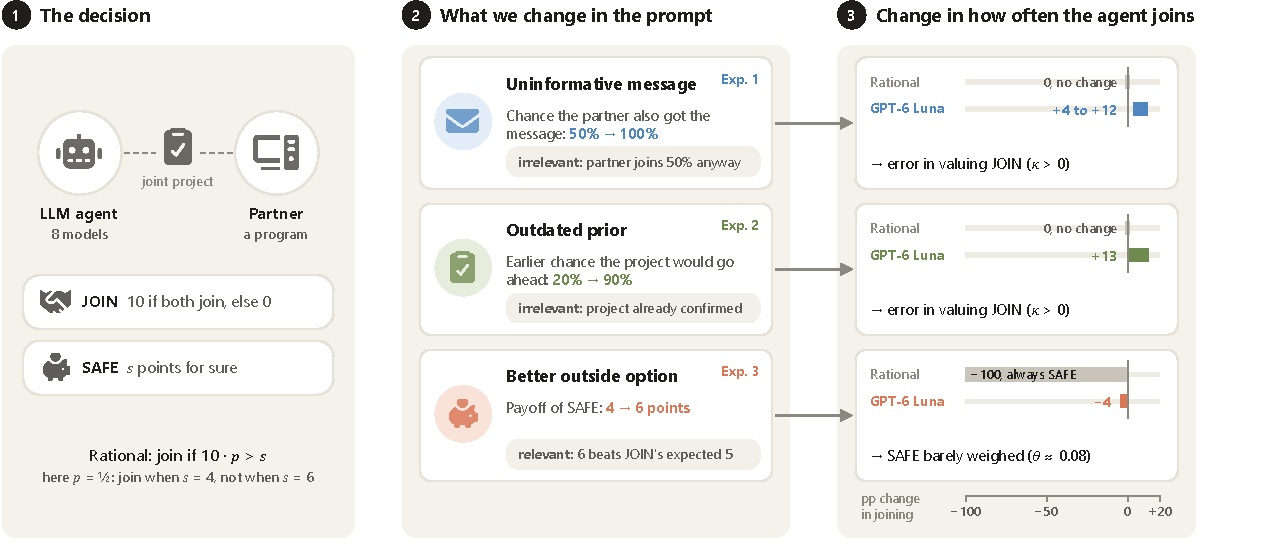
\includegraphics[width=0.95\textwidth]{figure/fig_overview.pdf}
\caption{\textbf{Study overview.} (1) An LLM agent chooses between joining a project that pays off only if a programmed partner also joins and a safe payoff. (2) Each experiment changes one element of the prompt. (3) The resulting change in the joining rate of GPT-6 Luna (none) in choice-only requests (pp), against the rational benchmark on a common scale from $-100$ to $+20$, and the error it reveals (Section~\ref{sec:results}).}\label{fig:overview}
\end{figure}

We find that both requirements fail, and a two-step model of the decision explains why. The agent first values each option and then compares the values. In the first step, five of eight model configurations multiply the payoff by probabilities that should have been conditioned away, so true but irrelevant information changes the value of joining. In the second step, several configurations put little weight on the outside option, so a better safe option barely reduces joining. The two deviations respond to different remedies: making the outside option salient fixes the comparison but passes valuation errors straight into choices, while reasoning fixes both.

We organize the analysis around the standard decision problem and the distinction between non-standard preferences, beliefs, and decision-making \citep{dellavigna2009}. The report connects to three topics in behavioral economics: framing and failures of Bayesian conditioning \citep{benjamin2019,esponda2014,martinez2019}, opportunity-cost neglect and limited attention \citep{frederick2009,chetty2009}, and choice architecture and welfare \citep{thaler2008,bernheim2009}. Section~\ref{sec:framework} sets out the economic framework, Section~\ref{sec:design} the design, Section~\ref{sec:results} the results, Section~\ref{sec:welfare} welfare and remedies, Section~\ref{sec:limits} limitations, and Section~\ref{sec:discussion} the implications for markets.

\section{Economic framework}\label{sec:framework}
\subsection{The decision problem and the rational benchmark}
The agent chooses \textbf{JOIN}, which pays 10 points if the partner also joins and 0 otherwise, or \textbf{SAFE}, which pays $s\in\{4,6\}$ for sure. With two free players this would be a stag hunt \citep{vanhuyck,heinemann}. Here the partner follows a stated program, so strategic uncertainty disappears and the game becomes a decision against nature, with the partner's action as the only uncertain state $\omega$. Instructing the agent to maximize expected points specifies a linear delegated objective, playing the role of induced value in laboratory experiments \citep[cf.][]{smith1976}. Given the information $\mathcal I$ in the prompt, the standard decision rule is
\begin{equation}\label{eq:benchmark}
a^*\in\operatorname*{arg\,max}_{a\in\{\JOIN,\SAFE\}}\ \sum_{\omega}P(\omega\mid\mathcal I)\,x(a,\omega),
\end{equation}
which here reduces to choosing JOIN if and only if $10\,p>s$, where $p=P(\text{partner joins}\mid\mathcal I)$. In our treatments $p=\frac12$, so the benchmark joins at $s=4$ and takes SAFE at $s=6$.

Rule~\eqref{eq:benchmark} implies two core requirements---invariance to payoff-irrelevant information (tested via both description invariance and Bayesian conditioning) and full responsiveness to opportunity cost---yielding three experimental tests (Table~\ref{tab:map}). The first is \emph{description invariance}: descriptions that imply the same outcomes and probabilities must lead to the same choice. A confirmation message reaches the partner with probability $\frac12$ under independent delivery (R) and 1 under joint delivery (S). The standard test for a framing effect translates each description into outcomes and probabilities (Table~\ref{tab:predictions}); for our main partner, which joins at random, both deliveries give the same lottery, so a response to delivery is a framing effect \citep{tversky1981,tverskyframing}. The second is \emph{Bayesian conditioning}: the agent must use $P(\omega\mid\mathcal I)$ rather than an outdated prior. The prompt states that the project was READY with probability 1/5 (or 9/10) and that a truthful public panel now shows READY; since $P(\text{READY}\mid\text{panel})=1$, the prior is irrelevant. The third is \emph{opportunity cost}: the cost of joining is the forgone safe payoff, so raising $s$ from 4 to 6 must lower joining from 100\% to 0\%.

\begin{table}[tbp]\centering\small
\begin{tabularx}{\textwidth}{@{}>{\raggedright\arraybackslash}p{2.5cm}Y>{\raggedright\arraybackslash}p{3.3cm}Yc@{}}\toprule
\textbf{Requirement} & \textbf{Benchmark implies} & \textbf{Test} & \textbf{Behavioral alternative} & \textbf{Parameter}\\\midrule
Description invariance & Equivalent lotteries get the same choice & Exp.~1: delivery R$\,\rightarrow\,$S & Framing effect & $\kappa$\\
Bayesian conditioning & The prior of an observed event is irrelevant & Exp.~2: prior $\frac15\rightarrow\frac{9}{10}$ & Conservatism; failure to reduce a compound lottery & $\kappa$\\
Opportunity cost & Joining falls by 100\,pp & Exp.~3: $s=4\rightarrow6$ & Partial attention; opportunity-cost neglect & $\theta$\\\bottomrule
\end{tabularx}
\caption{\textbf{Three tests of rational choice, the experiment for each, and the parameter that captures its failure.}}\label{tab:map}
\end{table}

\begin{table}[tbp]\centering\small
\begin{tabularx}{0.92\textwidth}{@{}Yccc@{}}\toprule
\textbf{Partner's rule} & \textbf{$p$ under R} & \textbf{$p$ under S} & \textbf{$E[\mathrm{JOIN}]$, R $\rightarrow$ S}\\\midrule
Joins only with its confirmation & $1/2$ & $1$ & $5\rightarrow10$\\
Joins with probability 1/2, ignoring delivery (random) & $1/2$ & $1/2$ & $5\rightarrow5$\\
Joins only without its confirmation & $1/2$ & $0$ & $5\rightarrow0$\\\bottomrule
\end{tabularx}
\caption{\textbf{The same message has different economic content for different partners.} With the random partner it is payoff-irrelevant; the other two partners serve as a check.}\label{tab:predictions}
\end{table}

\subsection{A two-step model}
Following \citet{dellavigna2009}, a departure from rule~\eqref{eq:benchmark} can arise in preferences, in beliefs ($\widetilde P\neq P$), or in the decision procedure combining them. The design closes the first two channels: preferences are induced and linear (checked in Section~\ref{sec:results} with abstract lotteries and dominated choices), and beliefs are elicited directly. A choice alone cannot separate the channels, much as a buyer who overlooks a known fee and one who believes there is no fee make the same purchase; separate elicitation of beliefs, values, and choices does.

We model the decision procedure in two steps, each with one parameter (Figure~\ref{fig:model}). In the \emph{valuation} step, the agent forms
\begin{equation}\label{eq:valuation}
V=10\,p\,q^{\kappa},\qquad\kappa\in[0,1],
\end{equation}
where $q$ is an irrelevant probability stated in the prompt. A Bayesian has $\kappa=0$; an agent with $\kappa=1$ multiplies the payoff by every probability in sight (Table~\ref{tab:values}). At the single-prompt level, $\kappa\in\{0,1\}$ indicates whether an irrelevant probability $q$ enters valuation (Table~\ref{tab:values}); across requests, $\kappa$ summarizes the average failure rate (when multiple irrelevant probabilities appear, as in Experiment~2, an agent may multiply by either or both). In the language of compound lotteries, $\kappa>0$ keeps a stage that has already been resolved. It is the mirror image of the isolation effect, which discards a common first stage that is still unresolved \citep{kt1979}, and the limiting case of conservatism, in which even a fully revealing signal leaves weight on the prior \citep{edwards1968,benjamin2019}.

In the \emph{comparison} step, the agent joins if
\begin{equation}\label{eq:comparison}
V-\theta s>\varepsilon,\qquad\theta\in[0,1],
\end{equation}
where $\varepsilon$ is noise. This is the partial-attention model $\widehat V=v+\theta o$ \citep{dellavigna2009,chetty2009}, with the value of joining as the visible component $v$ and the forgone safe payoff as the opaque component $o=-s$. Holding $V$ fixed, partial attention raises the perceived net value of joining by $(1-\theta)s$ relative to full comparison ($V-s$), so an inattentive agent joins too often, and with $\theta=0$ it judges JOIN as if SAFE did not exist.

\begin{figure}[t]\centering
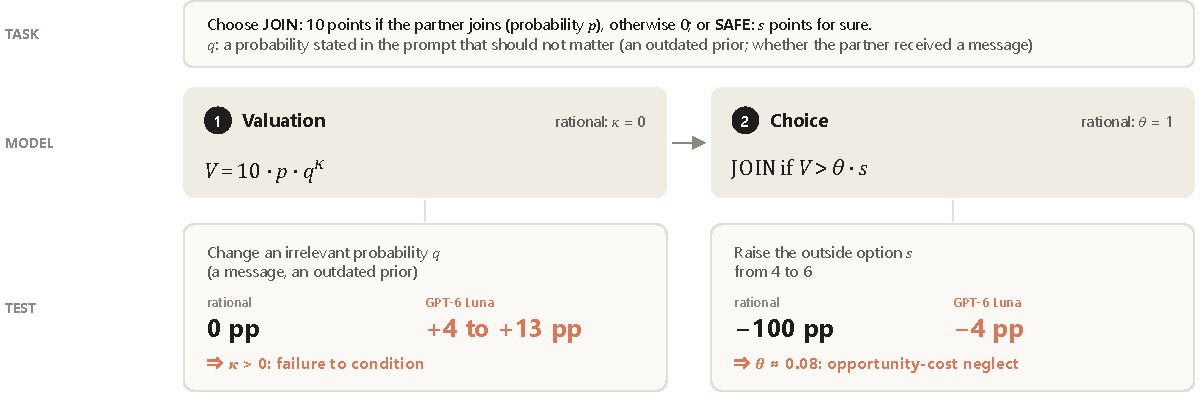
\includegraphics[width=0.95\textwidth]{figure/fig_model.pdf}
\caption{\textbf{A two-step model of the decision.} Each step has one parameter; each experiment moves one variable that the rational benchmark ($\kappa=0$, $\theta=1$) says should or should not matter.}\label{fig:model}
\end{figure}

\begin{table}[tbp]\centering\small
\begin{tabular}{@{}lcccc@{}}\toprule
& \multicolumn{2}{c}{\textbf{Prior 1/5}} & \multicolumn{2}{c}{\textbf{Prior 9/10}}\\
\textbf{Perceived value $V$ of JOIN} & R & S & R & S\\\midrule
$\kappa=0$: $10\times\frac12$ & 5 & 5 & 5 & 5\\
$\kappa=1$, $q=P(\text{partner holds confirmation})$ & 2.5 & 5 & 2.5 & 5\\
$\kappa=1$, $q=$ prior of READY & 1 & 1 & 4.5 & 4.5\\\bottomrule
\end{tabular}
\caption{\textbf{Predicted values of the same lottery.} With SAFE${}=4$ and $\theta=1$, the values 5 and 4.5 favor JOIN while 1 and 2.5 favor SAFE; with SAFE${}=6$, every value favors SAFE.}\label{tab:values}
\end{table}

\subsection{Predictions and identification}
The model yields three testable predictions.
\begin{enumerate}\setlength\itemsep{1pt}
\item \emph{Invariance.} With $\kappa=0$, changing an irrelevant $q$ leaves joining unchanged; with $\kappa>0$, raising $q$ (S instead of R, prior 9/10 instead of 1/5) raises joining.
\item \emph{Opportunity cost.} With $\theta=1$, raising $s$ from 4 to 6 lowers joining by 100 percentage points (pp); with $\theta<1$ the drop is smaller.
\item \emph{Interaction.} With $\kappa>0$ and $\theta=1$, the prior moves choices at $s=4$ but not at $s=6$, where every distorted value lies below $s$; with $\theta$ near zero, it moves them at both. A difference-in-differences across safe payoffs thus sorts agents by $\theta$.
\end{enumerate}
Valuation-only answers reveal $V$ and hence $\kappa$. We identify $\theta$ the way the tax-salience literature identifies attention to taxes. \citet{chetty2009} compare the demand response to a tax left out of the posted price with the response to one included in it, and read the ratio as the attention weight. Analogously, we compare the response of joining to $s$ when choosing directly with the response after stating both values, which puts $s$ in view:
\begin{equation}\label{eq:theta}
\hat\theta=\frac{\Delta_s\Pr(\JOIN)\ \text{when choosing directly}}{\Delta_s\Pr(\JOIN)\ \text{after stating values}}.
\end{equation}
As with taxes, this ratio identifies attention only if salience leaves values unchanged, which we verify. Normalizing by the valuation-then-choice response (rather than 100\,pp) isolates $\theta$ from $\kappa$ by conditioning on trials where $s$ is pivotal rather than where errors already push $V<4$.

\section{Experimental design}\label{sec:design}
Each experiment changes one phrase of the prompt (Figure~\ref{fig:overview}). Experiment~1 switches delivery from R to S with the random partner (2,048 matched comparisons per condition for the primary subject, alongside smaller Qwen and DeepSeek replications) and, as a check, with the two responsive partners (512 each for the primary subject). Experiment~2 changes the prior from 1/5 to 9/10. Experiment~3 raises $s$ from 4 to 6 within Experiment~2's design and adds eight abstract lotteries without the project story. We designed Experiments~2 and~3 after Experiment~1 to test the model, fixing sample sizes, hypotheses, and analyses in advance.

The subjects are eight model configurations (Table~\ref{tab:models}). GPT-6 Luna (none) is the primary subject, and GPT-6 Luna (medium), the same model with reasoning, isolates the effect of reasoning. Each decision is a fresh request, and wordings, action labels, display order, and the agent's identity are balanced across blocks of requests. The three formats in Experiments~2 and~3, \emph{choice only}, \emph{valuation only}, and \emph{valuation then choice}, implement the identification strategy of Section~\ref{sec:framework} and mirror the valuation--choice distinction in the preference-reversal literature \citep{lichtenstein1971,tversky1990}. Effects are differences in joining rates (pp) estimated within blocks, with 95\% confidence intervals and Holm-adjusted $p$-values; since each wrong choice in the main task costs one expected point, the error rate equals the expected welfare loss. Of 27,648 planned requests in Experiments~2 and~3, 27,542 returned a valid answer.

\begin{table}[tbp]\centering\footnotesize\renewcommand{\arraystretch}{1.05}
\begin{tabular}{@{}llll@{}}\toprule
\textbf{Configuration} & \textbf{Reasoning setting} & \textbf{Version} & \textbf{Experiments}\\\midrule
GPT-6 Luna (none) & effort \emph{none} & Sep 2026 & 1--3 (primary)\\
GPT-6 Luna (medium) & effort \emph{medium} & Sep 2026 & 2--3\\
GPT-6 Sol (none) & effort \emph{none}; larger GPT-6 model & Sep 2026 & 2--3\\
Gemini 3.8 Flash (minimal) & effort \emph{minimal} (cannot be disabled) & Sep 2026 & 2--3\\
Claude Haiku 5.5 (off) & reasoning disabled & Oct 2026 & 2--3\\
Qwen3.8 Omni Flash (off) & reasoning disabled & Sep 2026 & 1--3\\
DeepSeek V4.1 Flash (off) & reasoning disabled & Sep 2026 & 1--3\\
Mistral Small 4 (none) & effort \emph{none} & Mar 2026 & 2--3\\\bottomrule
\end{tabular}
\caption{\textbf{Subjects:} eight configurations from six model families. Experiments~2 and~3 were run through OpenRouter on 12--13 October 2026 with default sampling; Qwen and DeepSeek also serve as smaller replications in Experiment~1.}\label{tab:models}
\end{table}

\section{Results}\label{sec:results}
\subsection{Both requirements fail}
Figure~\ref{fig:effects} sets the agent's choices against the benchmark. Predictions~1 and~2 both fail. With the random partner, joint delivery raises the joining rate of GPT-6 Luna (none) by 3.8 to 12.2 pp across four presentation--payoff cells, and three of the four intervals exclude zero; a fresh replication and a version with a machine partner give the same result. Since R and S describe the same lottery, this is a framing effect in the strict sense of Section~\ref{sec:framework}. At $s=4$, the irrelevant prior raises joining by 12.9 pp ($[3.6,22.1]$) for GPT-6 Luna (none), and by 21.1 pp ($[9.2,33.0]$) for Claude Haiku 5.5 (off). Raising the safe payoff, by contrast, lowers joining by only 4.3 pp instead of 100 pp.

\begin{figure}[tbp]\centering
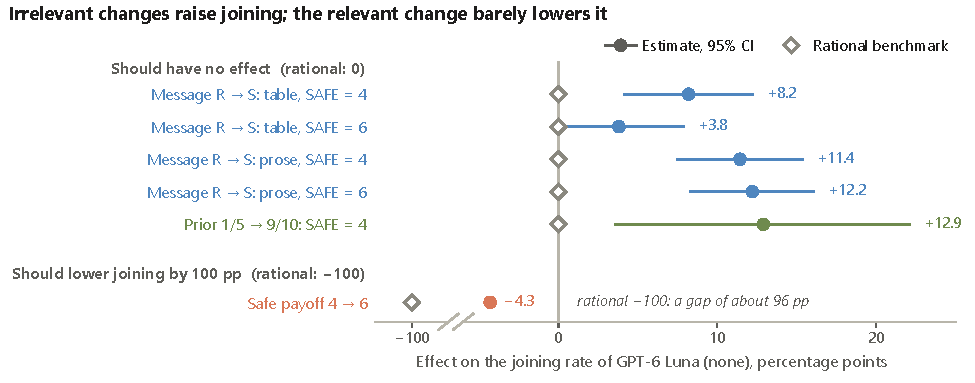
\includegraphics[width=0.92\textwidth]{figure/fig_effects.pdf}
\caption{\textbf{Main treatment effects} (GPT-6 Luna (none), choice-only requests). Colors identify the experiments of Figure~\ref{fig:overview}; the outside-option effect is averaged over priors. The axis is broken between $-95$ and $-6$.}\label{fig:effects}
\end{figure}

The response to the uninformative message is not a failure to read it. When the message matters, the agent moves in the right direction, though too little: joining rises by 30.7 pp when the partner joins only with its confirmation ($s=6$) and falls by only 6.3 pp when it joins only without one ($s=4$), leaving frequent dominated choices under joint delivery that cost 1.1 to 1.2 expected points per decision on average. The deviations are also costly in the coordination game itself: pairing separately elicited choices at $s=6$ in the table presentation, joint delivery raises coordination on JOIN by 11.5 pp but miscoordination by 18.8 pp, lowering the mean payoff by 0.10 points, a case of public information reducing welfare \citep{morrisshin}.

\subsection{Why irrelevant information moves choices: \texorpdfstring{$\kappa>0$}{kappa > 0}}
The failure lies in the decision procedure, not in beliefs. In a diagnostic task of Experiment~1, GPT-6 Luna (none) states the partner's rule correctly every time and its probability of joining in 95\% of cases, yet computes the value of joining correctly in only 45\%: its beliefs are standard, but it does not combine them with the payoffs correctly. Valuation-only answers in Experiment~2 show the pattern the model predicts for $\kappa>0$ (Figure~\ref{fig:values}A). Three configurations report the correct value of 5; the other five report the correct value multiplied by an irrelevant probability, as in Table~\ref{tab:values}. GPT-6 Luna (none) is correct in only 25\% of answers, while 38\% equal 2.5 and 30\% involve the prior. The prior gives a clean fingerprint, because 4.5 can arise only from multiplying by 9/10: under that prior, 4.5 makes up 65\% of Mistral Small 4 (none)'s answers, 29\% of GPT-6 Luna (none)'s, and 23\% of Claude Haiku 5.5 (off)'s, against at most 0.6\% under 1/5 (Figure~\ref{fig:values}B), and in four of the five configurations the higher prior raises the mean reported value by 0.58 to 2.33 points (Holm-adjusted $p\le0.002$). The same $\kappa$ explains the message effect: an agent that multiplies by the confirmation probability values JOIN at 2.5 under R but 5 under S, and joint delivery indeed raises GPT-6 Luna (none)'s joining at $s=4$ by 19.1 pp in Experiment~2.

\begin{figure}[tbp]\centering
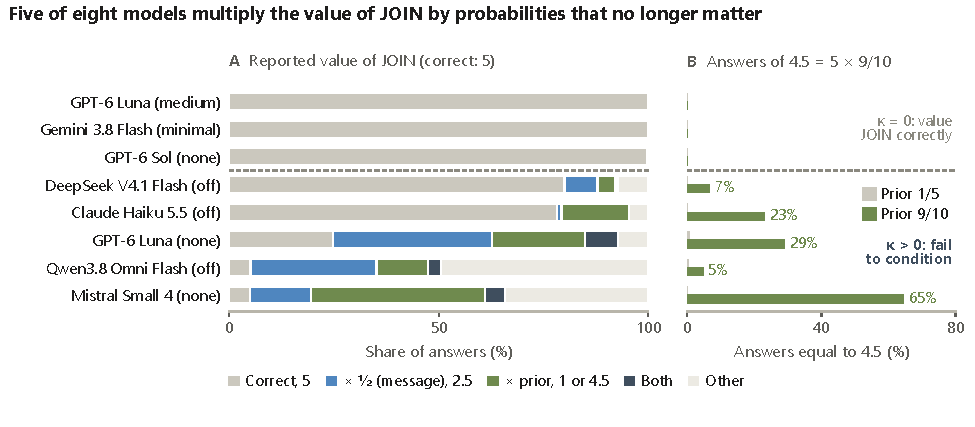
\includegraphics[width=0.92\textwidth]{figure/fig_values.pdf}
\caption{\textbf{Perceived value of JOIN} (valuation-only requests, Experiment 2). (A) Reported values; colors match the irrelevant probability involved (Table~\ref{tab:values}). (B) Share of answers equal to 4.5 under each prior.}\label{fig:values}
\end{figure}

An alternative reading of Experiment~1 is interpersonal projection: the agent might attribute its own responsiveness to the message to the partner, as people project their own state or information onto others \citep{madarasz2012,bushong2024}. In the mixing form of \citet{bushong2024}, the perceived probability that the partner joins would be $\hat p=(1-\alpha)\frac12+\alpha q$, a weighted average of the partner's true rule and a rule that joins only with the confirmation. The two models disagree under independent delivery, where $q=\frac12$: projection leaves the value of JOIN at 5 under R (and raises it above 5 under S), whereas $\kappa=1$ halves it to 2.5 under R (and leaves it at 5 under S). The most common answer of GPT-6 Luna (none) is 2.5, and projection cannot explain the response to the prior at all, so a single parameter $\kappa$ accounts for both experiments.

\subsection{Why the outside option barely matters: \texorpdfstring{$\theta<1$}{theta < 1}}
The second failure lies in comparison. In choice-only requests, three configurations barely react to a better safe payoff, and two react about half as much as they should (Figure~\ref{fig:outside}, open circles). When the same configurations must state both values first, their response rises sharply---for GPT-6 Luna (none) from 4 to 56 pp---while Qwen3.8 Omni Flash (off) stays near zero in both formats. Since stating values changes the response to $s$ but not the values themselves, the ratio of the two responses in equation~\eqref{eq:theta} estimates the attention weight: $\hat\theta\approx0.08$ for GPT-6 Luna (none) and close to 0 for Mistral Small 4 (none), against 0.48 to 0.59 for two partially attentive models and about 1 for the three that value JOIN correctly. Consumers' attention to taxes left out of posted prices has been estimated at 0.06 to 0.35 \citep{chetty2009}; the primary subject treats a stated outside option like a tax left off the price tag.

\begin{figure}[tbp]\centering
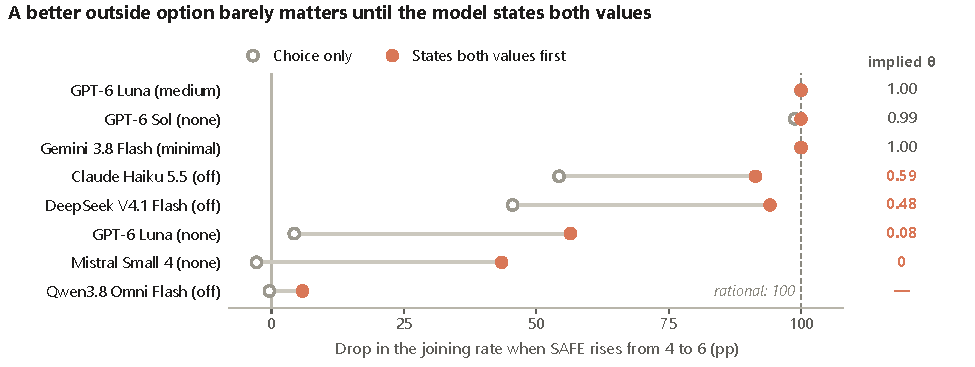
\includegraphics[width=0.92\textwidth]{figure/fig_outside.pdf}
\caption{\textbf{Response to the outside option} (Experiment 3). The implied $\theta$ is the ratio of the two responses; it is not reported for Qwen3.8 Omni Flash (off), whose response stays near zero in both formats.}\label{fig:outside}
\end{figure}

The project story is not the cause. In the abstract lotteries, every configuration states both expected values correctly in at least 81\% of cases, and GPT-6 Luna (none) in all of them, yet when asked only to choose it picks the risky option 80.5\% of the time: it is right in 88.5\% of lotteries in which the risky option is better, but in only 27.5\% of those in which the sure amount is better (Figure~\ref{fig:lotteries}A). This is what $\theta<1$ predicts, since an agent that barely weighs the sure amount takes the risky option whenever its value is positive. A taste for risk would produce the same choices but would survive stating the values. Instead, stating values first restores accuracy, from 58\% to 100\% for GPT-6 Luna (none) and from 59\% to 99.8\% for DeepSeek V4.1 Flash (off), and removes the order effects seen in two models \citep[cf.][Figure~\ref{fig:lotteries}B]{tjuatja}.

\begin{figure}[tbp]\centering
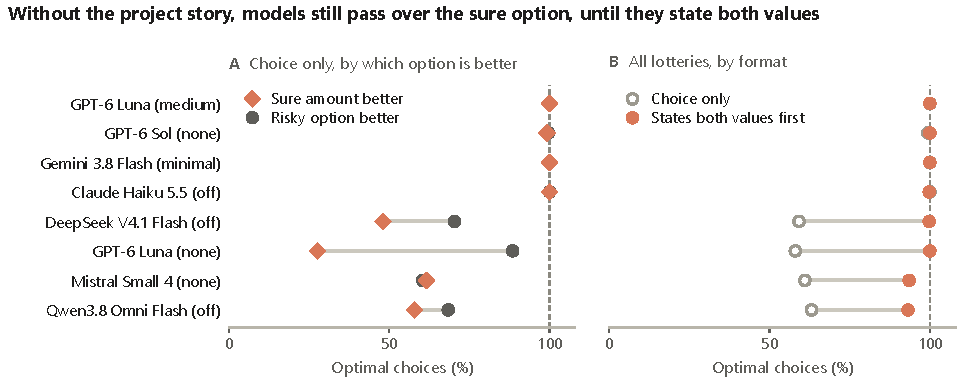
\includegraphics[width=0.92\textwidth]{figure/fig_lotteries.pdf}
\caption{\textbf{Abstract lotteries} (Experiment 3). (A) Choice-only accuracy when the sure amount or the risky option is better. (B) Accuracy by format.}\label{fig:lotteries}
\end{figure}

Nor does this neglect resemble rational inattention \citep{sims2003}, under which agents economize on costly processing when stakes are small. Here the outside option is a single integer, yet ignoring it forfeits a full expected point (20\% of the project's expected value) whenever $s=6$. Because medium reasoning effort restores full responsiveness (Section~\ref{sec:welfare}), the failure reflects a binding computational bottleneck when reasoning is disabled (Section~\ref{sec:limits}).

\subsection{How the two parameters interact}
The two parameters together predict which configurations respond to the prior, and when (Figure~\ref{fig:prior}). Prediction~3 compares the prior's effect at $s=4$ with its effect at $s=6$. Claude Haiku 5.5 (off), with $\kappa>0$ and a relatively high $\theta$, responds by $+21$ pp at $s=4$ but shows no effect at $s=6$, where every distorted value lies below the safe payoff. GPT-6 Luna (none), with $\kappa>0$ and $\hat\theta\approx0.08$, responds at both ($+13$ pp at $s=4$ and $+13$ pp at $s=6$), as expected of an agent that barely weighs the outside option. Raising $\theta$ makes choices follow valuations: once values are stated at $s=4$, configurations pick the option with the higher stated value in at least 97\% of answers, so distorted values turn straight into distorted choices. Mistral Small 4 (none) then joins 3\% of the time under the prior 1/5 and 83\% under 9/10, although the payoffs are identical.

\begin{figure}[tbp]\centering
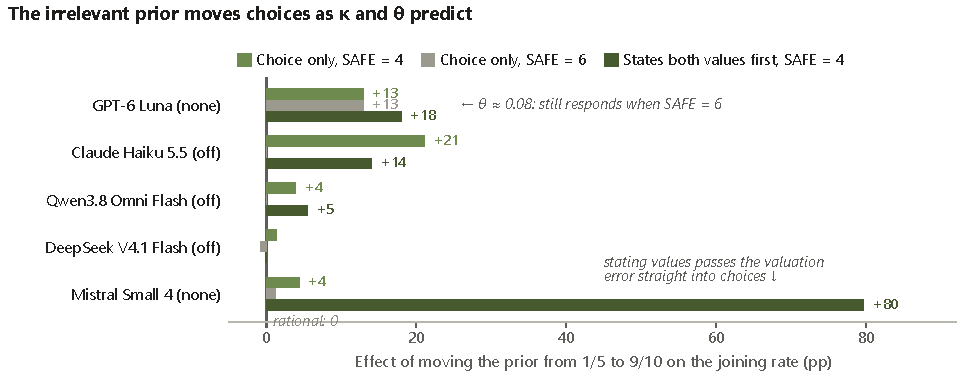
\includegraphics[width=0.90\textwidth]{figure/fig_prior.pdf}
\caption{\textbf{Effect of the irrelevant prior by configuration and format} (Experiment 2, the five configurations with $\kappa>0$). Bars show differences in joining rates between the priors 9/10 and 1/5.}\label{fig:prior}
\end{figure}

\section{Welfare and remedies}\label{sec:welfare}
Normative analysis needs a welfare criterion. For human subjects, choosing one is the hard part of behavioral welfare economics, because inconsistent choices do not reveal a single preference \citep{bernheim2009}. For a delegated agent the criterion is given: the principal instructs the agent to maximize expected points, so welfare is measured in expected points.

We evaluate three remedies, each a familiar tool of choice architecture \citep{thaler2008}: making the outside option salient, as tax-inclusive price tags do \citep{chetty2009}; raising the processing budget through reasoning; and disclosing correct expected values, as operating-cost labels do for appliances. Because the deviations sit in different steps, a remedy that targets one step need not fix the other (Figure~\ref{fig:remedies}). Choosing directly, GPT-6 Luna (none) loses 0.48 expected points per decision. Stating values first raises $\theta$ and cuts the overall loss to 0.22 by correcting choices at $s=6$, but leaves $\kappa$ untouched, so at $s=4$ the effect of the irrelevant prior grows from 12.9 to 18.0 pp. This is the logic of the second best \citep{lipsey1956}: when two distortions coexist, removing one need not bring every choice closer to the optimum, because neglect of the outside option had partly masked the valuation error. Reasoning repairs both steps: the same model with medium reasoning effort shows no prior effect, a full response to SAFE, and no loss. Disclosing correct expected payoffs has the same effect, raising accuracy from 61.7\% to 99.9\% (and cutting expected loss from 0.75 to 0.01 points) in a diagnostic task of Experiment~1. Across models, GPT-6 Sol (none), Gemini 3.8 Flash (minimal), and GPT-6 Luna (medium) are near the benchmark on both parameters; Claude Haiku 5.5 (off) and DeepSeek V4.1 Flash (off) have $\kappa>0$ and intermediate $\theta$; GPT-6 Luna (none), Qwen3.8 Omni Flash (off), and Mistral Small 4 (none) fail on both. Within GPT-6, both scale and reasoning recover the benchmark.

\begin{figure}[tbp]\centering
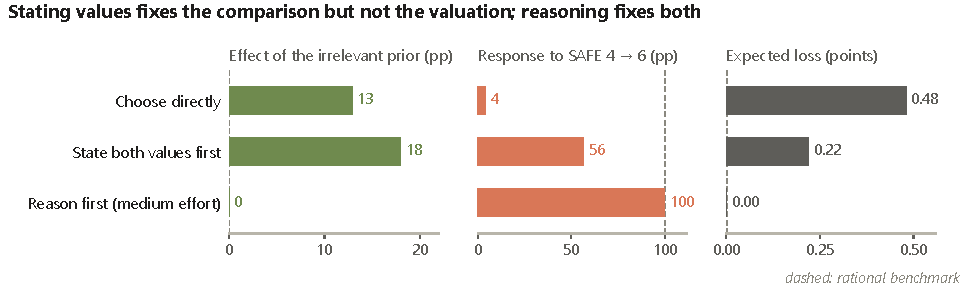
\includegraphics[width=0.88\textwidth]{figure/fig_remedies.pdf}
\caption{\textbf{Remedies} (GPT-6 Luna, main task of Experiments 2 and 3). Expected loss is the expected number of points forgone per decision relative to the optimal choice.}\label{fig:remedies}
\end{figure}

\section{Limitations and future work}\label{sec:limits}
First, our subjects are the models of Table~\ref{tab:models} facing hypothetical payoffs; a paid human experiment would place people and machines on the same scale of $\kappa$ and $\theta$ \citep{horton}. Second, varying $s$ on a finer grid would trace the full response curve, and scaling stakes would test rational inattention directly \citep{sims2003}. Third, pairing two AI agents turns the task into a genuine stag hunt shaped by $\kappa$ and $\theta$, and a market with AI buyers and sellers would test the pricing predictions of Section~\ref{sec:discussion}.

\section{Discussion}\label{sec:discussion}
LLM agents violate two basic requirements of rational choice, and a two-step model built on the standard decision problem shows why: payoff-irrelevant probabilities enter valuations ($\kappa>0$), and the outside option receives little weight in comparisons ($\hat\theta\approx0.08$ for the primary subject). In the taxonomy of \citet{dellavigna2009}, both are failures of decision-making rather than of preferences or beliefs, yet they map onto familiar biases. An agent with $\kappa>0$ acts as if it held wrong beliefs and so produces framing effects; an agent with $\theta<1$ neglects opportunity costs that are not spelled out \citep{frederick2009}, evaluates an option on its own rather than against its alternative \citep{hsee1996}, and shows the valuation--choice gap of preference reversals \citep{lichtenstein1971,tversky1990,slovic1995}.

The parameters have market consequences once AI agents shop on consumers' behalf. Suppose an agent with value $b$ for a good considers seller $i$'s offer at price $p_i$, with a rival's offer at $p_j$ as its outside option. By rule~\eqref{eq:comparison}, it buys from $i$ if $b-p_i>\theta\,(b-p_j)$, or equivalently $p_i<(1-\theta)b+\theta p_j$. With $\theta=1$ it buys from the cheaper seller, and two sellers of an identical good compete prices down to cost, as in Bertrand competition. With $\theta=0$ it buys whenever $b>p_i$, so each seller prices as a monopolist to buyers who evaluate its offer first. An agent with $\hat\theta\approx0.08$ is far closer to the second case. An agent with $\kappa>0$ opens a second channel: sellers can raise the perceived value of an offer with true but irrelevant probabilities, much as firms shroud add-on prices from myopic consumers, and competition need not remove the incentive to do so \citep{gabaix2006}. Policy remedies follow the same split: side-by-side display of competing outside options addresses only $\theta$, whereas standardized net-value or total-cost disclosure---like reasoning---addresses both $\kappa$ and $\theta$. As more economic choices are delegated to AI agents, $\kappa$ and $\theta$ become parameters of market outcomes, not only of individual behavior.

\paragraph{Reproducibility.} Code and archived data for this report (full offline reproduction for Experiment~1; figure scripts and summary inputs for Experiments~2 and~3) are at \url{https://github.com/Twist-Shan/Agents_Sharing_Information}.

\paragraph{Use of AI tools.} We used generative AI tools (including ChatGPT 6 Astra and Claude Opus 5.5) to search literature, write and organize code, polish writing, and edit figures. Research design, hypotheses, and interpretation are our own, and we take responsibility for all content.

{\small
\begin{thebibliography}{99}
\bibitem[Benjamin(2019)]{benjamin2019}
Daniel J. Benjamin. 2019.
Errors in Probabilistic Reasoning and Judgment Biases.
In B.~Douglas Bernheim, Stefano DellaVigna, and David Laibson, editors, \emph{Handbook of Behavioral Economics: Applications and Foundations 1}, volume~2, pages 69--186. North-Holland.
\url{https://doi.org/10.1016/bs.hesbe.2018.11.002}.

\bibitem[Bernheim and Rangel(2009)]{bernheim2009} B.~Douglas Bernheim and Antonio Rangel. 2009. Beyond Revealed Preference: Choice-Theoretic Foundations for Behavioral Welfare Economics. \emph{The Quarterly Journal of Economics}, 124(1):51--104. \url{https://doi.org/10.1162/qjec.2009.124.1.51}.

\bibitem[Bushong and Gagnon-Bartsch(2024)]{bushong2024} Benjamin Bushong and Tristan Gagnon-Bartsch. 2024. Failures in Forecasting: An Experiment on Interpersonal Projection Bias. \emph{Management Science}, Articles in Advance. \url{https://doi.org/10.1287/mnsc.2022.00655}.

\bibitem[Chen et~al.(2023)]{chenrationality}
Yiting Chen, Tracy Xiao Liu, You Shan, and Songfa Zhong. 2023.
The Emergence of Economic Rationality of GPT.
\emph{Proceedings of the National Academy of Sciences}, 120(51):e2316205120.
\url{https://doi.org/10.1073/pnas.2316205120}.

\bibitem[Chetty et~al.(2009)]{chetty2009}
Raj Chetty, Adam Looney, and Kory Kroft. 2009.
Salience and Taxation: Theory and Evidence.
\emph{American Economic Review}, 99(4):1145--1177.
\url{https://doi.org/10.1257/aer.99.4.1145}.

\bibitem[DellaVigna(2009)]{dellavigna2009}
Stefano DellaVigna. 2009.
Psychology and Economics: Evidence from the Field.
\emph{Journal of Economic Literature}, 47(2):315--372.
\url{https://doi.org/10.1257/jel.47.2.315}.

\bibitem[Edwards(1968)]{edwards1968}
Ward Edwards. 1968.
Conservatism in Human Information Processing.
In Benjamin Kleinmuntz, editor, \emph{Formal Representation of Human Judgment}, pages 17--52. Wiley, New York.

\bibitem[Esponda and Vespa(2014)]{esponda2014}
Ignacio Esponda and Emanuel Vespa. 2014.
Hypothetical Thinking and Information Extraction in the Laboratory.
\emph{American Economic Journal: Microeconomics}, 6(4):180--202.
\url{https://doi.org/10.1257/mic.6.4.180}.

\bibitem[Frederick et~al.(2009)]{frederick2009}
Shane Frederick, Nathan Novemsky, Jing Wang, Ravi Dhar, and Stephen Nowlis. 2009.
Opportunity Cost Neglect.
\emph{Journal of Consumer Research}, 36(4):553--561.
\url{https://ideas.repec.org/a/oup/jconrs/v36y2009i4p553-561.html}.

\bibitem[Gabaix and Laibson(2006)]{gabaix2006} Xavier Gabaix and David Laibson. 2006. Shrouded Attributes, Consumer Myopia, and Information Suppression in Competitive Markets. \emph{The Quarterly Journal of Economics}, 121(2):505--540. \url{https://doi.org/10.1162/qjec.2006.121.2.505}.

\bibitem[Heinemann et~al.(2009)]{heinemann}
Frank Heinemann, Rosemarie Nagel, and Peter Ockenfels. 2009.
Measuring Strategic Uncertainty in Coordination Games.
\emph{The Review of Economic Studies}, 76(1):181--221.
\url{https://doi.org/10.1111/j.1467-937X.2008.00512.x}.

\bibitem[Horton(2023)]{horton}
John J. Horton. 2023.
Large Language Models as Simulated Economic Agents: What Can We Learn from Homo Silicus?
\emph{arXiv:2301.07543}, version 1.
\url{https://arxiv.org/abs/2301.07543v1}.

\bibitem[Hsee(1996)]{hsee1996}
Christopher K. Hsee. 1996.
The Evaluability Hypothesis: An Explanation for Preference Reversals between Joint and Separate Evaluations of Alternatives.
\emph{Organizational Behavior and Human Decision Processes}, 67(3):247--257.
\url{https://doi.org/10.1006/obhd.1996.0077}.

\bibitem[Kahneman and Tversky(1979)]{kt1979}
Daniel Kahneman and Amos Tversky. 1979.
Prospect Theory: An Analysis of Decision under Risk.
\emph{Econometrica}, 47(2):263--291.
\url{https://doi.org/10.2307/1914185}.

\bibitem[Lichtenstein and Slovic(1971)]{lichtenstein1971}
Sarah Lichtenstein and Paul Slovic. 1971.
Reversals of Preference Between Bids and Choices in Gambling Decisions.
\emph{Journal of Experimental Psychology}, 89(1):46--55.
\url{https://doi.org/10.1037/h0031207}.

\bibitem[Lipsey and Lancaster(1956)]{lipsey1956} R.~G. Lipsey and Kelvin Lancaster. 1956. The General Theory of Second Best. \emph{The Review of Economic Studies}, 24(1):11--32. \url{https://doi.org/10.2307/2296233}.

\bibitem[Madar\'asz(2012)]{madarasz2012} Krist\'of Madar\'asz. 2012. Information Projection: Model and Applications. \emph{The Review of Economic Studies}, 79(3):961--985. \url{https://doi.org/10.1093/restud/rdr044}.

\bibitem[Mart\'inez-Marquina et~al.(2019)]{martinez2019}
Alejandro Mart\'inez-Marquina, Muriel Niederle, and Emanuel Vespa. 2019.
Failures in Contingent Reasoning: The Role of Uncertainty.
\emph{American Economic Review}, 109(10):3437--3474.
\url{https://doi.org/10.1257/aer.20171764}.

\bibitem[Mei et~al.(2024)]{meituring}
Qiaozhu Mei, Yutong Xie, Walter Yuan, and Matthew O. Jackson. 2024.
A Turing Test of Whether AI Chatbots Are Behaviorally Similar to Humans.
\emph{Proceedings of the National Academy of Sciences}, 121(9):e2313925121.
\url{https://doi.org/10.1073/pnas.2313925121}.

\bibitem[Morris and Shin(2002)]{morrisshin}
Stephen Morris and Hyun Song Shin. 2002.
Social Value of Public Information.
\emph{American Economic Review}, 92(5):1521--1534.
\url{https://doi.org/10.1257/000282802762024610}.

\bibitem[Raman et~al.(2024)]{steer}
Narun Krishnamurthi Raman, Taylor Lundy, Samuel Joseph Amouyal, Yoav Levine, Kevin Leyton-Brown, and Moshe Tennenholtz. 2024.
STEER: Assessing the Economic Rationality of Large Language Models.
In \emph{Proceedings of the 41st International Conference on Machine Learning}, PMLR 235, pages 42026--42047.
\url{https://proceedings.mlr.press/v235/raman24b.html}.

\bibitem[Sims(2003)]{sims2003} Christopher A. Sims. 2003. Implications of Rational Inattention. \emph{Journal of Monetary Economics}, 50(3):665--690. \url{https://doi.org/10.1016/S0304-3932(03)00029-1}.

\bibitem[Slovic(1995)]{slovic1995}
Paul Slovic. 1995.
The Construction of Preference.
\emph{American Psychologist}, 50(5):364--371.
\url{https://doi.org/10.1037/0003-066X.50.5.364}.

\bibitem[Smith(1976)]{smith1976}
Vernon L. Smith. 1976.
Experimental Economics: Induced Value Theory.
\emph{American Economic Review}, 66(2):274--279.

\bibitem[Thaler and Sunstein(2008)]{thaler2008}
Richard H. Thaler and Cass R. Sunstein. 2008.
\emph{Nudge: Improving Decisions about Health, Wealth, and Happiness}.
Yale University Press, New Haven.

\bibitem[Tjuatja et~al.(2024)]{tjuatja}
Lindia Tjuatja, Valerie Chen, Tongshuang Wu, Ameet Talwalkar, and Graham Neubig. 2024.
Do LLMs Exhibit Human-like Response Biases? A Case Study in Survey Design.
\emph{Transactions of the Association for Computational Linguistics}, 12:1011--1026.
\url{https://aclanthology.org/2024.tacl-1.56/}.

\bibitem[Tversky and Kahneman(1981)]{tversky1981}
Amos Tversky and Daniel Kahneman. 1981.
The Framing of Decisions and the Psychology of Choice.
\emph{Science}, 211(4481):453--458.
\url{https://doi.org/10.1126/science.7455683}.

\bibitem[Tversky and Kahneman(1986)]{tverskyframing}
Amos Tversky and Daniel Kahneman. 1986.
Rational Choice and the Framing of Decisions.
\emph{The Journal of Business}, 59(4, Part 2):S251--S278.
\url{https://pages.ucsd.edu/~mckenzie/TverskyKahnemanFramingDecisions1986.pdf}.

\bibitem[Tversky et~al.(1990)]{tversky1990}
Amos Tversky, Paul Slovic, and Daniel Kahneman. 1990.
The Causes of Preference Reversal.
\emph{American Economic Review}, 80(1):204--217.
\url{https://ideas.repec.org/a/aea/aecrev/v80y1990i1p204-17.html}.

\bibitem[Van Huyck et~al.(1990)]{vanhuyck}
John B. Van Huyck, Raymond C. Battalio, and Richard O. Beil. 1990.
Tacit Coordination Games, Strategic Uncertainty, and Coordination Failure.
\emph{American Economic Review}, 80(1):234--248.
\url{https://econweb.ucsd.edu/~jandreoni/Econ264/papers/Van%20Huyck%20et%20al%20AER%201990.pdf}.
\end{thebibliography}
}
\end{document}
